
\begin{frame}{What is Deep RL?}
Deep RL is the combination of \textbf{reinforcement learning (RL)} with \textbf{deep learning}

\begin{itemize}
\item \textbf{Reinforcement learning} is about solving problems by \textbf{trial and error}
\item \textbf{Deep learning} is about using \textbf{deep neural networks} to solve problems
\item $\Longrightarrow$ \textbf{Deep reinforcement learning} trains deep neural networks with trial and error
\end{itemize}

\twocolumns{0.4}{0.6}{
\begin{figure}
\centering
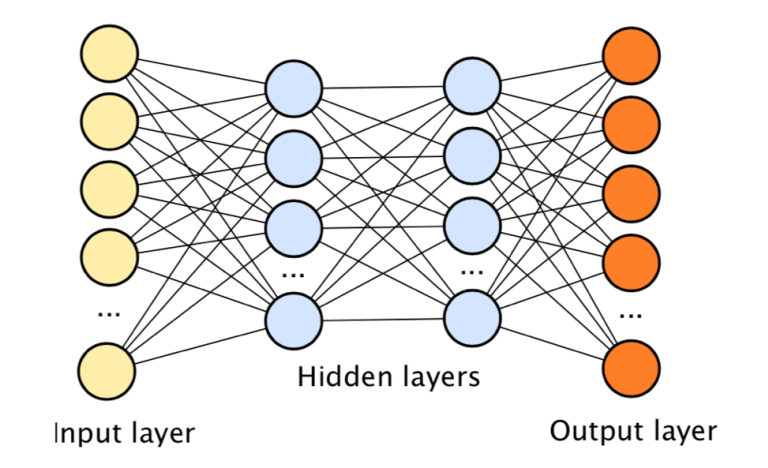
\includegraphics[width=\textwidth]{deep-neural-networks}
\end{figure}
}{
\begin{figure}
\centering
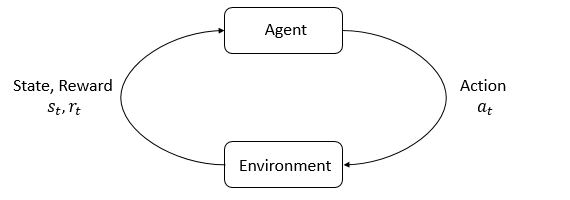
\includegraphics[width=\textwidth]{agent-interaction-loop}
\end{figure}
}
\begin{center}
Deep neural network\footnote{Deep neural network image from Gary Marcus} and RL interaction loop
\end{center}
\end{frame}

\begin{frame}{When would you want to use RL?}

RL is useful when
%
\begin{itemize}
\item you have a sequential decision-making problem
\item you do \textbf{not} know the optimal behavior already\footnotemark[1]
\item but you can still evaluate whether behaviors are good or bad
\end{itemize}

\vspace{3em}

That is, 

\begin{center}
\boxed{
\textbf{RL is useful when evaluating behaviors is easier than generating them}
}
\end{center}

\footnotetext[1]{Critical difference from supervised learning!}

\end{frame}

\begin{frame}{When would you want to use deep learning?}

\twocolumns{0.5}{0.5}{
Deep learning is useful when
%
\begin{itemize}
\item you want to approximate a function
\item function requires ``intelligence"
\item inputs and/or outputs are high-dimensional
\item lots of data is available
\end{itemize}

\vspace{2em}

This includes \textbf{tons} of problems!
%
\begin{itemize}
\item image recognition / facial classification
\item sentiment analysis
\item neural machine translation
\item automatic speech recognition
\item etc.
\end{itemize}
}{
\begin{figure}
\centering
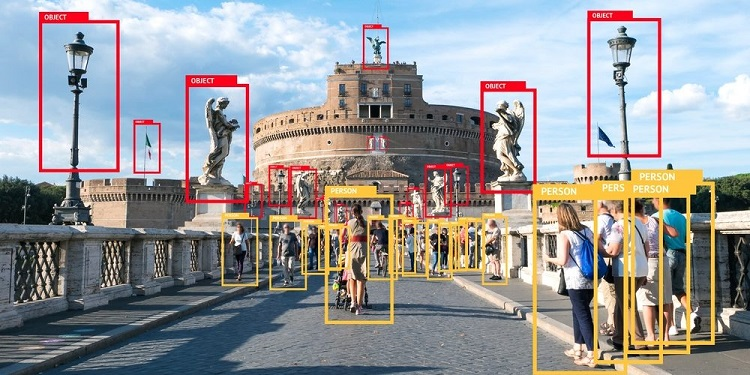
\includegraphics[width=0.85\textwidth]{dl-object-detection}
\caption{Object detection\footnotemark[1]}
\end{figure}
\begin{figure}
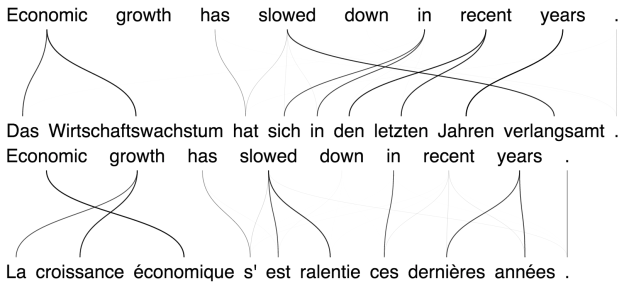
\includegraphics[width=0.85\textwidth]{dl-neural-machine-translation}
\caption{Machine translation\footnotemark[2]}
\end{figure}
}

\footnotetext[1]{Intel Software,``A Closer Look at Object Detection, Recognition and Tracking"}
\footnotetext[2]{Nvidia Developer Blog, ``Introduction to Neural Machine Translation with GPUs"}

\end{frame}

\begin{frame}{When would you want to use deep RL?}
Deep RL can...
\begin{itemize}
\item Play video games from raw pixels
\item Control robots in simulation and in the real world
\item Play Go, Dota, and Starcraft at superhuman levels
\end{itemize}

\begin{columns}
\begin{column}{0.33\textwidth}
    \begin{center}
     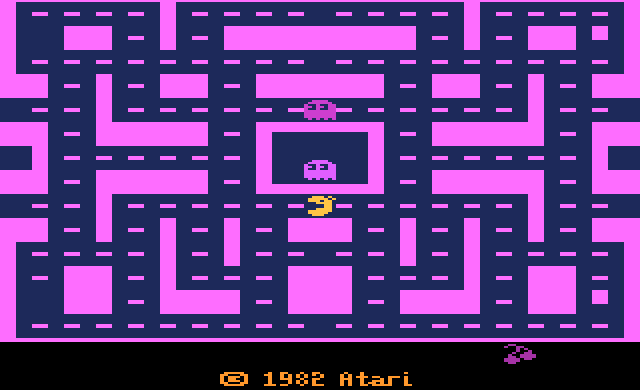
\includegraphics[width=0.9\textwidth]{ms_pacman}

     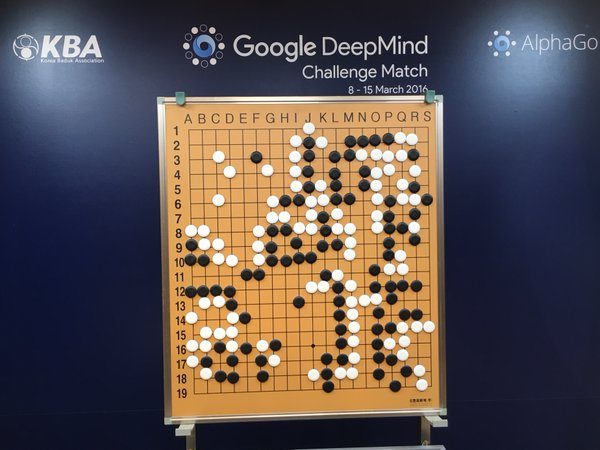
\includegraphics[width=0.9\textwidth]{alphago}
     \end{center}
\end{column}
\begin{column}{0.67\textwidth}
\movie[width=0.9\textwidth, autostart, loop]{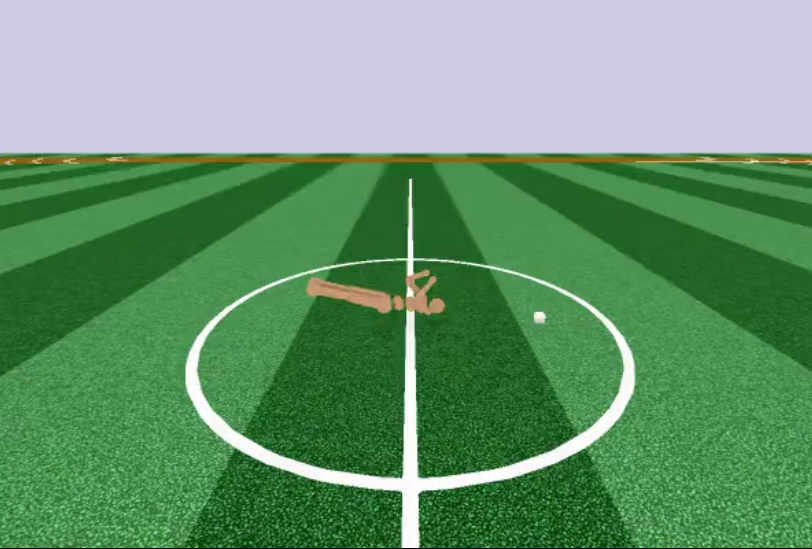
\includegraphics[width=0.9\textwidth]{knocked_down_standup}}{images/knocked-over-stand-up.mp4}
\end{column}
\end{columns}
\end{frame}